\chapter{MNIST}\label{ch:mnist}

\openepigraph{AI is a tool. The choice about how it gets deployed is ours.}{Oren Etzioni}

 
The MNIST database of handwritten digits, available from this page, has a training set of 60,000 examples, and a test set of 10,000 examples. This is a well known data-set, and is targeted by both MLPs and Convolutional Neural Network. We thus found  this to be an excellent starting point for LogicNet. 
We do some topology exploration on this data-set, and study a wide array of architectural decisions in detail. \\

While exploring our search space, we begun with MLPs on the MNIST data-set. To gain insights, we had to ascertain a few things which would make our search more effective. Some of the notable observations while attempting to gain insights on how to discover good topologies were as follows. Note that the observations below are specific to the MNIST data-set and only valid for MLPs.
\begin{itemize}
    \item For MLPs, going from 2 hidden layers to 3 hidden layers still has benefits, i.e. the intermediate layers do not learn an identity function.
    \item In our tests, a drop-out at the input layer gives very slight benefits.
    \item Drop-out in the intermediate layers with A Priori Random Fixed Sparsity causes accuracy to deteriorate irrespective of the size of the hidden layer, or bit-width.
    \item ADAM and SGD as optimizers give very similar accuracy results.
    \item Increasing bit-width from 1 to 2 is beneficial, but not at the cost of neuron fan-in in terms of synapses. 
    \item Increasing number of neurons in a hidden layer is beneficial up-to 1024, after which the utility diminishes. 
    \item The last layer cannot have low per-neuron fan in. It causes serious detriments to accuracy of the network. For this reason unless mentioned otherwise; \textbf{all our experiments for MNIST report models with the final layer dense}.
\end{itemize}

To study how our Analytical LUT cost varies with accuracy, we trained an array of models on the MNIST dataset, all of which were 3 Layer MLPs. \cref{fig:3lmlplutacc} Shows that there is consistently a lower bound in terms of LUTs for the same performance. It is worth nothing that the Y axis is logarithmic, which means that a poor choice of Neuron Fan-In with a sub-optimal Bit-Width and Connectivity configuration can be very detrimential. 

\begin{table}
    \begin{sidecaption}[MNIST MLP Model List]{%
        This table describes the models in detail, it also gives the layerwise breakdown of LUTs (From the Analytical LUT Cost Model) and the accuracy. These models have been trained with Fixed A-Priori Sparsity, and is just for topology exploration. 
    }[mnist:tab:mnistmodels]
\begin{threeparttable}
\begin{tabular}{lrrrrrrrr}
\hline
HL              & BW & X & LUTL1   & LUTL2 & LUTL3 & LUTL4    & LUTs & Accuracy \\ \hline
(512)$\times$1  & 2  & 6 & 87k   & 43.9k & -  & -           & 131k   & 95.62    \\
(1024)$\times$1 & 2  & 5 & 43k   & 87.7k & -  & -           & 130k   & 95.86         \\
(2048)$\times$2 & 2  & 5 & 86k   & 175k    & -    & -     & 261k     & 94.77          \\ 
(512)$\times$2  & 2  & 6 & 87k   & 87k    & 43.5k    & -    & 217.6k & 96.58     \\ 
(1024)$\times$2 & 2  & 5 & 43k   & 43k    & 87k    & -     & 173k    & 96.85         \\ 
(2048)$\times$2 & 2  & 5 & 86k   & 86k    & 174k    & -     & 345.8k & 96.96         \\ 
(512)$\times$3  & 2  & 6 & 87k   & 87k    & 87k    & 43.5k  & 304.6k & 96.53   \\ 
(1024)$\times$3 & 2  & 5 & 43k   & 43k    & 43k    & 87k  &  215.9k  & 96.92    \\ 
(2048)$\times$3 & 2  & 5 & 86k   & 86k    & 86k & 173.8k   &  431.8k & 97.41          \\ \hline
\end{tabular}
\end{threeparttable}
\end{sidecaption}
\end{table}

\begin{figure}[h]
    \centering
    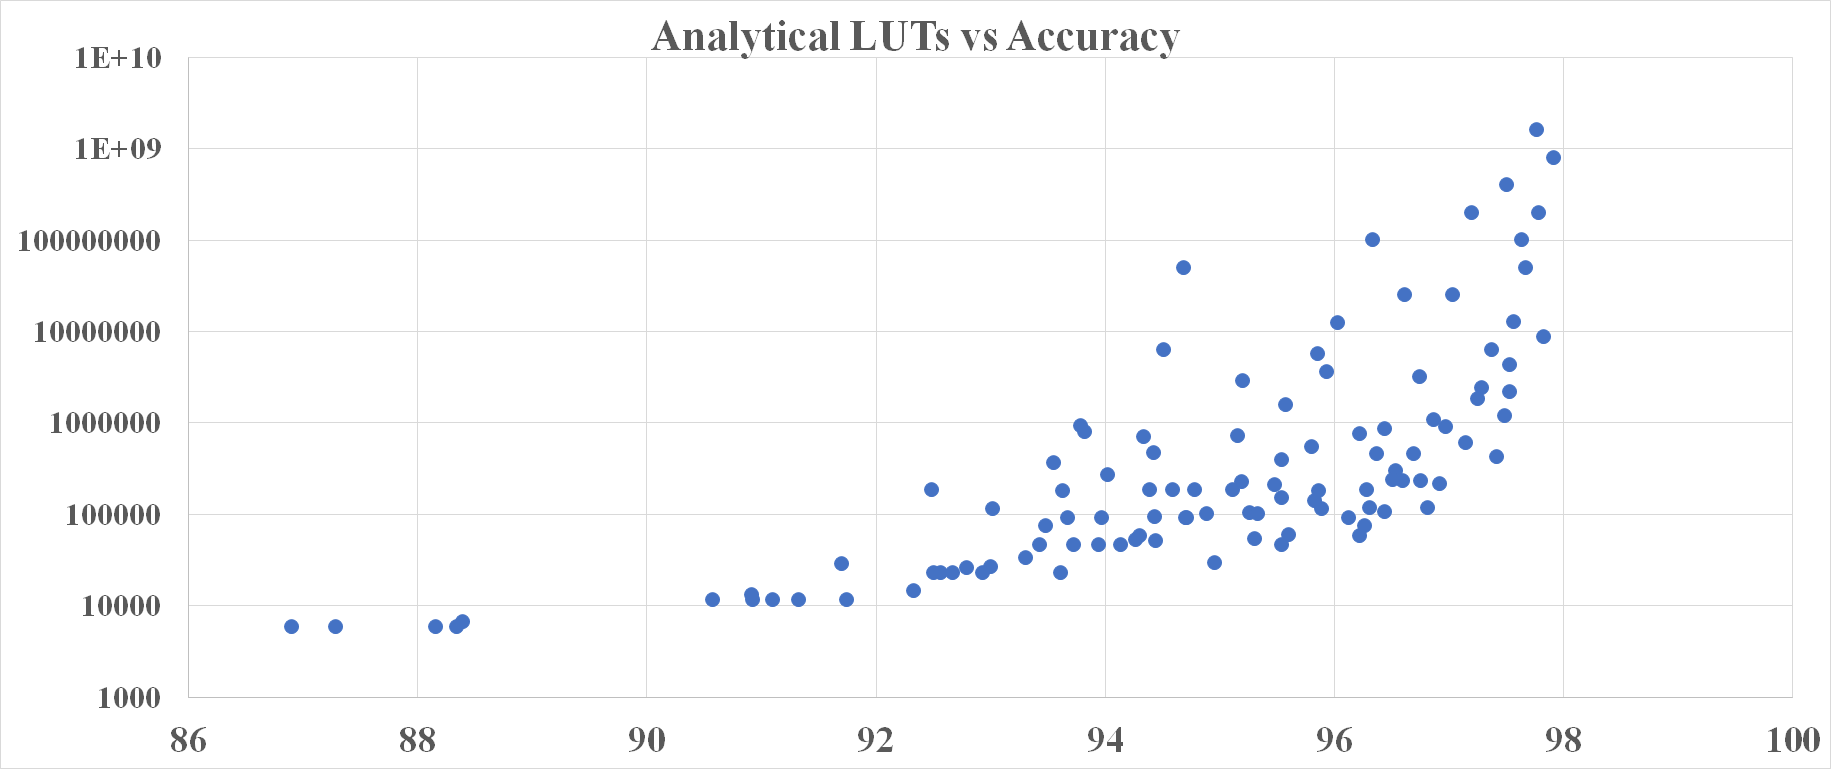
\includegraphics[width=330pt]{figures/bison/3lmlplutacc.png}
    \caption{Analytical LUT cost vs. Accuracy for a 3 Layer MLP on the MNIST Data-Set.}
    \label{fig:3lmlplutacc}
\end{figure}

\begin{figure}[h]
    \centering
    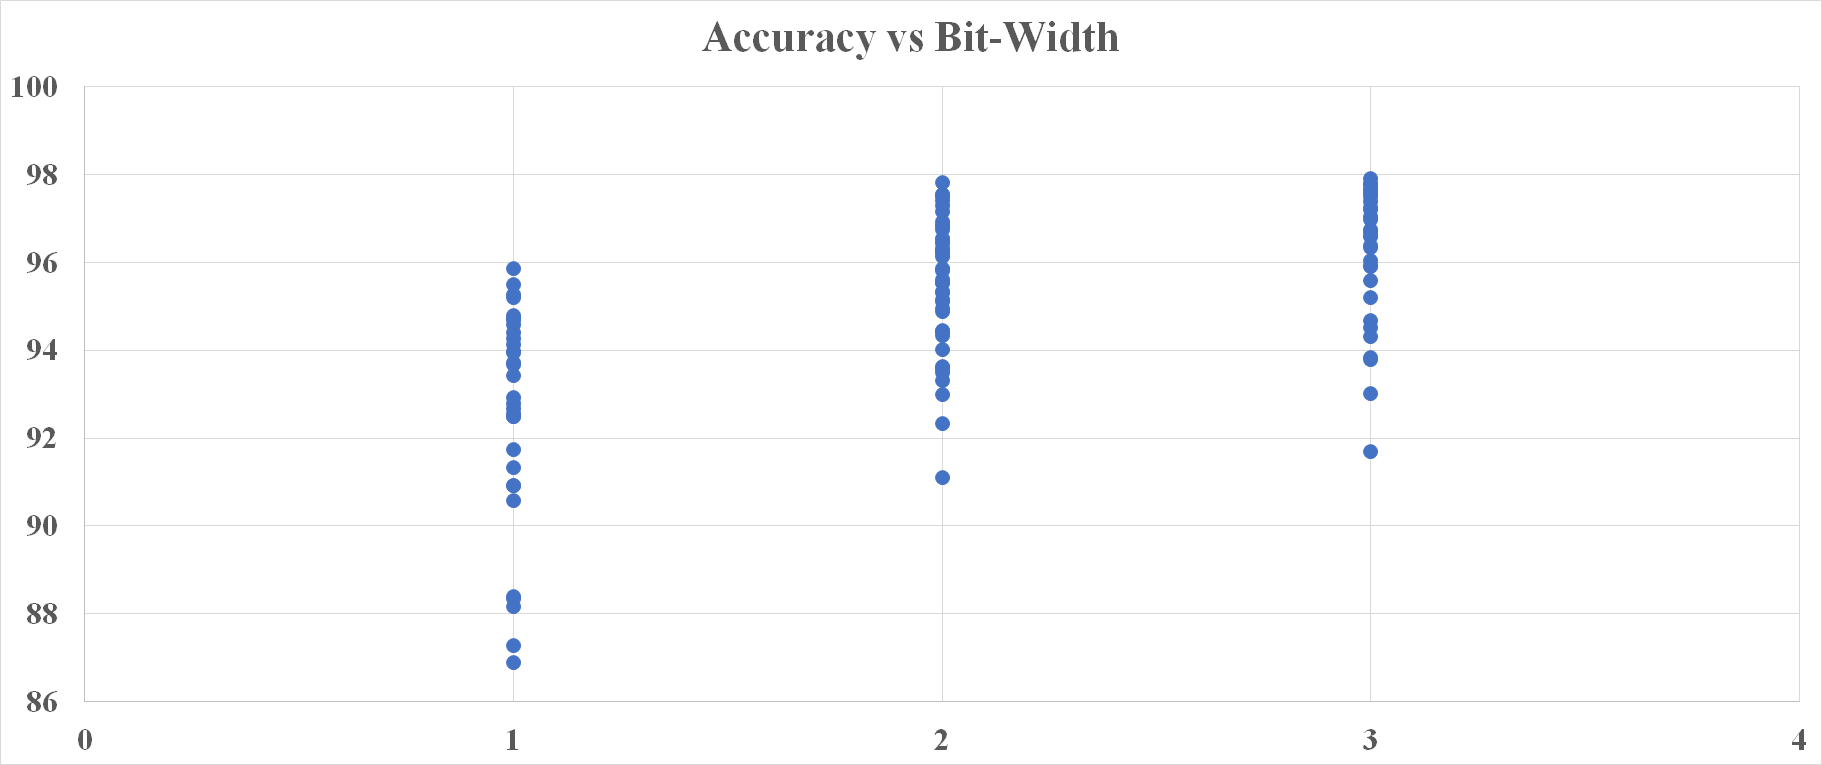
\includegraphics[width=330pt]{figures/bison/3lmnistaccbw.png}
    \caption{Accuracy vs. Bit-Width for a 3 Layer MLP on the MNIST Data-Set.}
    \label{fig:3lmnistaccbw}
\end{figure}


From \cref{mnist:tab:mnistmodels}, we gain further insights into the role of depth and width of the network for accuracy on MNIST. We see an upward trend in accuracy as we increase the depth of the neural network. Further, we can see the benefits of increasing the Bit-Width for a 3 Layer MLP on the  MNIST data-set from \cref{fig:3lmnistaccbw}. \\

% \newpage

\newthoughtpar{Iterative and Learned Sparsity}
In our tests, A-Priori Fixed Random Sparsity consistently gave poor accuracies when compared to Iterative and Learned Sparsity. This may be due to the fact that the MNIST data-set is flattening an Image and thus has definite structure in the flattened input. Initializing random connectivity is thus detrimential, whereas iterative and learned sparsity methods are able to discover important connections. From \cref{mnist:tab:iterativevmomentumvrandom}, we can be relatively confident that Iterative Pruning is the best strategy to train models with such sparsity. Momentum Sparsity gives better results than A-Priori Fixed Sparsity and requires almost the same amount of resources and time. Iterative Pruning takes about 10$\times$ longer to train, based on your pruning rates.

\begin{table}
    \begin{sidecaption}[Accuracy vs Pruning Techniques]{%
        This table depicts the accuracies for models trained with A-Priori Fixed Sparsity, Momentum Sparsity and Iterative Pruning techniques. 
    }[mnist:tab:iterativevmomentumvrandom]
\begin{threeparttable}
\begin{tabular}{lrrrr}
\hline
Model & A-Priori Fixed Sparsity & Momentum Sparsity & Iterative Pruning \\ \hline
A     &  97.32             &          97.68        & \textbf{97.78}     \\
B     &  97.12             &          97.39    & \textbf{97.75}    \\
C     &  96.58             &          97.22    & \textbf{97.63}          \\    \hline 
    \end{tabular}
\end{threeparttable}
\end{sidecaption}
\end{table}

\newthoughtpar{Skip Connections}
Due to the nature of LogicNet, we can introduce 'Skip Connections' to a neural network. As long as the per neuron fan-in remains the same, the LUT cost remains the same. What influence this has on Place and Route and the complexity it introduces is beyond the scope of this thesis. \\
As evidenced by \cref{mnist:tab:skiparch}, we see notable increase in accuracy with  no overhead in LUT cost. Thus, this can be an important avenue to explore in the future.


\begin{table}
    \begin{sidecaption}[Skip Connections on MLPs]{%
        We observe the accuracy of 3 Layer MLPs with Skip Connections. 
    }[mnist:tab:skiparch]
\begin{threeparttable}
\begin{tabular}{lrrrr}
\hline
Model & No Skip & 1 Skip & 2 Skips            \\ \hline
A     &  92.86  & 93.89  & \textbf{94.66}     \\
B     &  94.47  & 95.03  & \textbf{95.18}     \\
C     &  95.71  & \textbf{95.88}  & 95.78      \\
D     &  94.67  & 95.24  & \textbf{95.51}      \\    \hline 
    \end{tabular}
\end{threeparttable}
\end{sidecaption}
\end{table}

\newthoughtpar{Convolutional Neural Networks}
To get better performance, we need to use topologies which are tailored for images. An exploration of how such sparsity translated to computer vision tasks is very important. As discussed before, we use 'Sparse Depthwise Separable Convolution' to facilitate realistic mapping of convolutions to LUTs. We also use heavy quantization. \cref{mnist:tab:degrademnist} Shows how accuracy is affected as we change the topology and its bit-precision and sparsity. We test the accuracy of 4 variants of the same topology. The 'FP' being the full precision model with vanilla convolutions, 'FP\_DW' being the full precision model but with Depthwise Separable Convolutions. 'FP\_X\_DW' further introduces sparsity in the depthwise separable convolution and finally 'QUANT\_X\_DW' quantizes the sparse depthwise separable convolutional model. \cref{mnist:tab:degrademnist} seems to indicate that quantization causes the most notable degradation in accuracy. 

\begin{table}
    \begin{sidecaption}[Bringing Convolutions to LogicNet]{%
        Taking a specific model and observing its accuracy as we change the Pruning, Quantization and Convolution method.
    }[mnist:tab:degrademnist]
\begin{threeparttable}
\begin{tabular}{lrrrrrrrr}
\hline
Model        & A     & B     & C     \\ \hline
FP           & 98.68 & 98.96 & 99.15 \\
FP\_DW       & 98.34 & 97.7  & 98.6  \\
FP\_X\_DW    & 97.25 & 97.93 & 97.41 \\
QUANT\_X\_DW & 96.84 & 97.59 & 95.89 \\ \hline
\end{tabular}
\end{threeparttable}
\end{sidecaption}
\end{table}

\begin{table}
    \begin{sidecaption}[Accuracy and LUT cost of CNNs on the MNIST data-set]{%
        This table describes the models in detail, it also gives the Analytical LUT Cost and the accuracy. These models have been trained with Fixed A-Priori Sparsity, and is just for topology exploration. BW Stands for Bit-Width, X stands for the (Xk, Xs). Xk is the kernel sparsity, and Xs is the sparsity of the pointwise operation in Depthwise Separable Convolution.
    }[mnist:tab:convmnist]
\begin{threeparttable}
\begin{tabular}{lrrrr}
\hline
Model & BW & X      & LUTs & Accuracy \\ \hline
A     & 2  & (5,5)  & 145k & 95.87    \\
B     & 2  & (3,5)  & 345k & 97.47    \\
C     & 2  & (5, 4) & 769k & 97.59    \\
D     & 2  & (5, 6) & 420k & 97.57    \\ \hline
\end{tabular}
\end{threeparttable}
\end{sidecaption}
\end{table}

% \newpage

\newthoughtpar{Convolution Skip Connections}
After testing skip connections on MLPs, it only made sense to explore what its scope is for convolutional neural networks. We present our findings similar to before, with 1 skip connection and 2 skip connections. The activation of the first convolutional layer and second convolutional layer is concatenated to the activation of the second convolutional layer and activation of the final convolutional layer respectively. 
From \cref{mnist:tab:convskip}, we see some accuracy improvements. We do not discuss these skip connections in too much detail as it is beyond the scope of this thesis. It is however a direction worth exploring. 

\begin{table}[h]
    \begin{sidecaption}[Skip Connections on MNIST Convolutional models.]{%
        We observe the accuracy of a 3 Layer LogicNet style Convolutional Neural Network with Skip Connections. 
    }[mnist:tab:convskip]
\begin{threeparttable}
\begin{tabular}{lrrrr}
\hline
Model & No Skip & 1 Skip & 2 Skips            \\ \hline
A     & 96.74 & 96.93  & \textbf{96.94 }    \\
B     & 97.08 & 97.56  & \textbf{97.57}     \\
C     & 96.94 & \textbf{97.36}  & 97.13      \\  \hline 
    \end{tabular}
\end{threeparttable}
\end{sidecaption}
\end{table}

% /*
% Introduction
% The need for accelerators
%     CPUs, GPUs, ASICs, FPGAs.
% Background
%     FPGA and HW/SW Co-Design
%     Mapping Neurons to Hardware
%       Sparsity
%           Expander, Iterative, Momentum
%       Quantize
%           Activation brevitas
%           Non Linear
% LogicNet: A Library for Mapping HBBs to NEQs
%     Introduction
%     Components
%       Linear
%       Convolutions
%     Design Automation
%       TruthTableGen
%       VerilogGen
%       Synthesis
% Testing LogicNet
%     LogicNet4HEP
%       Introduction
%       Models
%     MNIST 
%       Models
% Concluding Remarks
%     Research Questions
%     Conclusion
% */